\documentclass{article}
\usepackage[english]{babel}
\usepackage[utf8x]{inputenc}
\usepackage{amsmath}
\usepackage{graphicx}


\title{12.1 Tests}
\author{chris }
\date{October 2017}

\begin{document}


\noindent BECA / Huson / 12.1 IB Math SL \qquad \qquad Name:\\
18 October 2018
\subsection*{Homework: Differential calculus}
Show working for all problems. State answers exactly or to three significant figures.\\*[5pt]

Take the derivative of each function

\begin{enumerate}

\item $f(x) = x^2 - 2x + 11$.
\item $f(x)=\sqrt{x}$
\item $f(x)=x^2 e^x$
\item $f(x)=(x^2-5)\ln{x}$
\item $\displaystyle f(x)=\frac{\sin{x}}{x^3}$
\item $f(x)=\cos{(1-x^2)}$

\item Let $f(x)=a(x-h)^2+k$. The vertex of the graph of $f$ is at $(2,3)$ and the graph passes through $(1,7)$.
\begin{enumerate}
    \item Write down the value of $h$ and $k$.
    \item Find the value of $a$.
\end{enumerate}

\item A function is given as $y = x^2 + kx -8$.
\begin{enumerate}
    \item Find $\displaystyle \frac {dy}{dx}$.
	\item If the gradient of this function is 2 when $x$ is 3, show that $k=-4$.
	\item Find the equation of the line tangent to the function through the point $(4, -8)$.
\end{enumerate}

\item An arithmetic sequence is given by 5, 8, 11, $\ldots$.
\begin{enumerate}
    \item Write down the value of $d$.
	\item Find
	\begin{enumerate}
	    \item $u_{100}$
	    \item $S_{100}$
	\end{enumerate}
	\item Given that $u_n = 1502$, find the value of $n$.
\end{enumerate}

\newpage
\item Let $f(x)=px^3+px^2+qx$.
\begin{enumerate}
    \item Find $f'(x)$.
	\item Given that $f'(x) \geq 0$, show that $p^2 \leq 3pq$.
\end{enumerate}

\item	Given the function $f(x) = \ln{x^2}+kx+5, x \neq 0$.
\begin{enumerate}
    \item Find $f'(x)$.
	\item The function $f(x)$ has a local maximum at $x=2$. Show that $k=-1$
\end{enumerate}

\item Given the function $\displaystyle f(x) = \frac{1}{x^2-4} +3$.
\begin{enumerate}
    \item For what values of $x$ is the function undefined?
    \item Hence and otherwise, write down the equations of the two vertical asymptotes and one horizontal asymptote.
    \item Find $f'(x)$.
    \item Show that there is a local maximum or minimum at $x=0$
    \item Find the equation of the normal to the function when $x = 1$.

\end{enumerate}

\item The position of an object is given by the function $s=e^{\sin t}-1$, for $0 \leq t \leq 5$.
\begin{enumerate}
    \item On the grid below, sketch the graph of $s$. (set your calculator to radians)
    \begin{figure}[!ht]
        \centering
        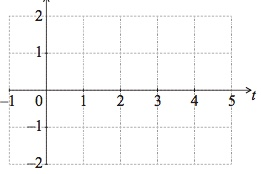
\includegraphics[width=0.6\textwidth]{sine-graph.jpeg}
    \end{figure}
    \item Write down the positive $t$-intercept.
    \item Find the velocity of the object, $v(t)$.
\end{enumerate}


\end{enumerate}

\end{document}
